% !TeX spellcheck = da_DK
\documentclass[../main.tex]{subfiles}


\begin{document}

\chapter{Introduktion}
\section{Problemet og dets perspektiv}
\subsection{Reinforcement Learning som }
%TODO: Tilføj henvisninger til nogle af påstandene
Reinforcement Learning er en af de mest generelle læringsparadigmer i maskinlæring: 
Den enkle opsætning med en agent, et miljø og maksimering af kumulativ skalar-belønning indfører få antagelser om problemets natur og gør sammenligninger til menneskelig læring og fantasier om kunstig generel intelligens fristende.
Når de helt store fremtidsperspektiver lægges til side, er der ofte praktiske mål som selvkørende biler, produktionsrobotter og andre autonome systemer, som bliver set som Reinforcement Learnings potentiale.
Sådanne fysiske agenter i kontinuerte, dynamiske miljøer falder oplagt ind, når man tænker på Reinforcement Learnings formulering og dets familieforhold til kontrolteori, der har rig tradition for styring af fysiske systemer. 

Det er dog unødvendigt begrænsende at se dette lovende maskinlæringsparadigme som dybt forbundet til det kontinuerte og fysiske: Mængden af praktiske beslutningsproblemer er stor og alsidig og der findes vigtige opgaver med helt andre modelleringsudfordringer end f.eks. bevægelse af et robotlegeme.

Diskret optimering er et dybt og velstuderet felt indenfor anvendt matematik og datalogi med klassiske problemer som \textit{Traveling Salesman}, grundlæggende datastrukturer som grafer og matroider og vigtige ingeniørpraktiske anvendelser som operationsanalyse, computationel kemi og planlægningssystemer. 
Disse problemer, der kan udmynte sig i kombinatorisk optimering vha. heltalsprogrammering eller optimering under bibetingelser, har ofte dybe strukturer beskrevet af abstrakt algebra herunder gruppeteori.
\\
\\
I denne rapport vil Reinforcement Learnings generaliserbarhed undersøges ved at bruge det som løsningsmetode til et sådant ikke-trivielt diskret problem, der konventionelt løses med algoritmer fra gruppeteorien.
Det større mål er altså at opnå erfaringer ved at bruge Reinforcement Learning på det kombinatoriske beslutningsproblem, perspektivere det til domænespecifikke løsningsstragier og undersøge udfordringerne med Reinforcement Learning i et stort udfaldsrum. 

\subsection{Rubiks Terning}

Rubiks terning er et lille, kombinatorisk legetøj opfundet af den ungarske billedhugger og professor i arkitektur Ernö Rubik i 1974. Med 350 mio. solgte terninger regnes den seksfarvede terning som det bedst sælgende legetøj og har fortsat en dedikeret fanskare organiseret i \textit{World Cube Association}, der afholder \textit{speedcuber}-arrangementer og deler praktiske løsningsalgoritmer \cite{RubiksWiki}. 
\begin{figure}[H]
	\centering 
	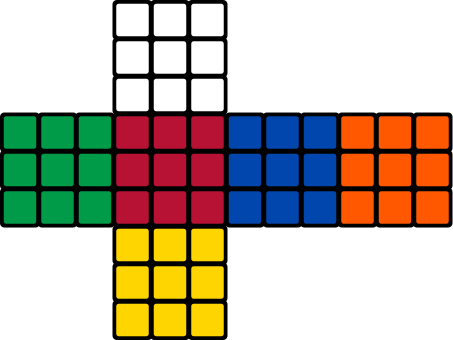
\includegraphics[width=.5\linewidth]{wiki_rubiks_colors}
	\caption{Illustration of de seks farvede sider i en 3x3 Rubiks terning.\protect\footnotemark}
\end{figure}
\footnotetext{Billede: Wikimedia Commons på \url{https://en.wikipedia.org/wiki/File:Rubik\%27s_cube_colors.svg}}
Terningen findes i et utal 





\cite{SolvingNature}



-- Problem challenge: Large state space, single goal state 

-- Do without domain knowledge

-- Learn to solve planning problems

-- Rooted in group theory: application of machine learning methods to mathematics

\cite{RubiksMedium}
-- Example of use of reinforcement learning in combinatorial optimization which also includes problems such as travelling salesman, protein folding simulation, resource allocation

\section{State of the Art}
\cite{RubiksMedium}
Siden Erno Rubik opfandt sin berømte terning i 1974, er der blevet opfundet adskillige løsningsalgoritmer.
Disse kan overordnet set inddeles i to grupper:
Gruppeteoribaserede algoritmer, fx Kociembas algoritme, og brute force-algoritmer med udgangspunkt i skræddersyede heurestikker.
De forskellige algoritmer har forskellige fordele og ulemper;
nogle skal være lette for mennesker at løse, mens andre er designet til såkaldte speed cubers, der skal løse terningen med så få træk som muligt;
nogle er optimerede til lavt hukommelsesforbrug og andre til at kunne løses hurtigt af computere.\\
\\
En ny tilgang til løsningsalgoritmer og diskrete problemer generelt er dyb reinforcement learning.
-- Algorithmic ways to solve the cube can be divided into group theory algorithms such as Kociemba's algorithm and brute force algorithms combined with crafted heuristics

--



\cite{SolvingNature}
-- Puzzle specific pattern databases solves these rubiks well


-- DeepCubeA solves all test configurations and generalizes to other puzzles

-- A shortest path (non-learned) solver is iterative deepening A* search with heuristic from puzzle specific pattern database and uses large data base and group theory 

\subsection{DeepCubeA}
\cite{SolvingNature}
-- Combines DL with approximate value iteration and batch weighted A* search

-- DNN approximates cost-to-go and is called deep approximate value iteration. It only looks one step ahead but multi-step lookahead  and MC tree search was not found to be better

-- DeepCubeA builds on another implementation which was based on policy and Monte Carlo tree search 

-- Learned cost-to-go function then used as heuristic to find path to goal state using weighted A* search

-- DNN: Two fully connected hidden layers, four residual blocks, linear output unit
%Scrambling between 100 and 10000 times + included furthest states.
\end{document}